\subsection{Prérequis}

Pour utiliser ChromaCase, vous aurez besoin de

\begin{itemize}
	\item Un Piano avec une connectivité MIDI
	\item Un ordinateur,ou une tablette ou smartphone Android  avec une connectivité pour brancher votre piano (généralement USB)
	\item Une connection Internet
\end{itemize}


\subsection{Fonctionnement}
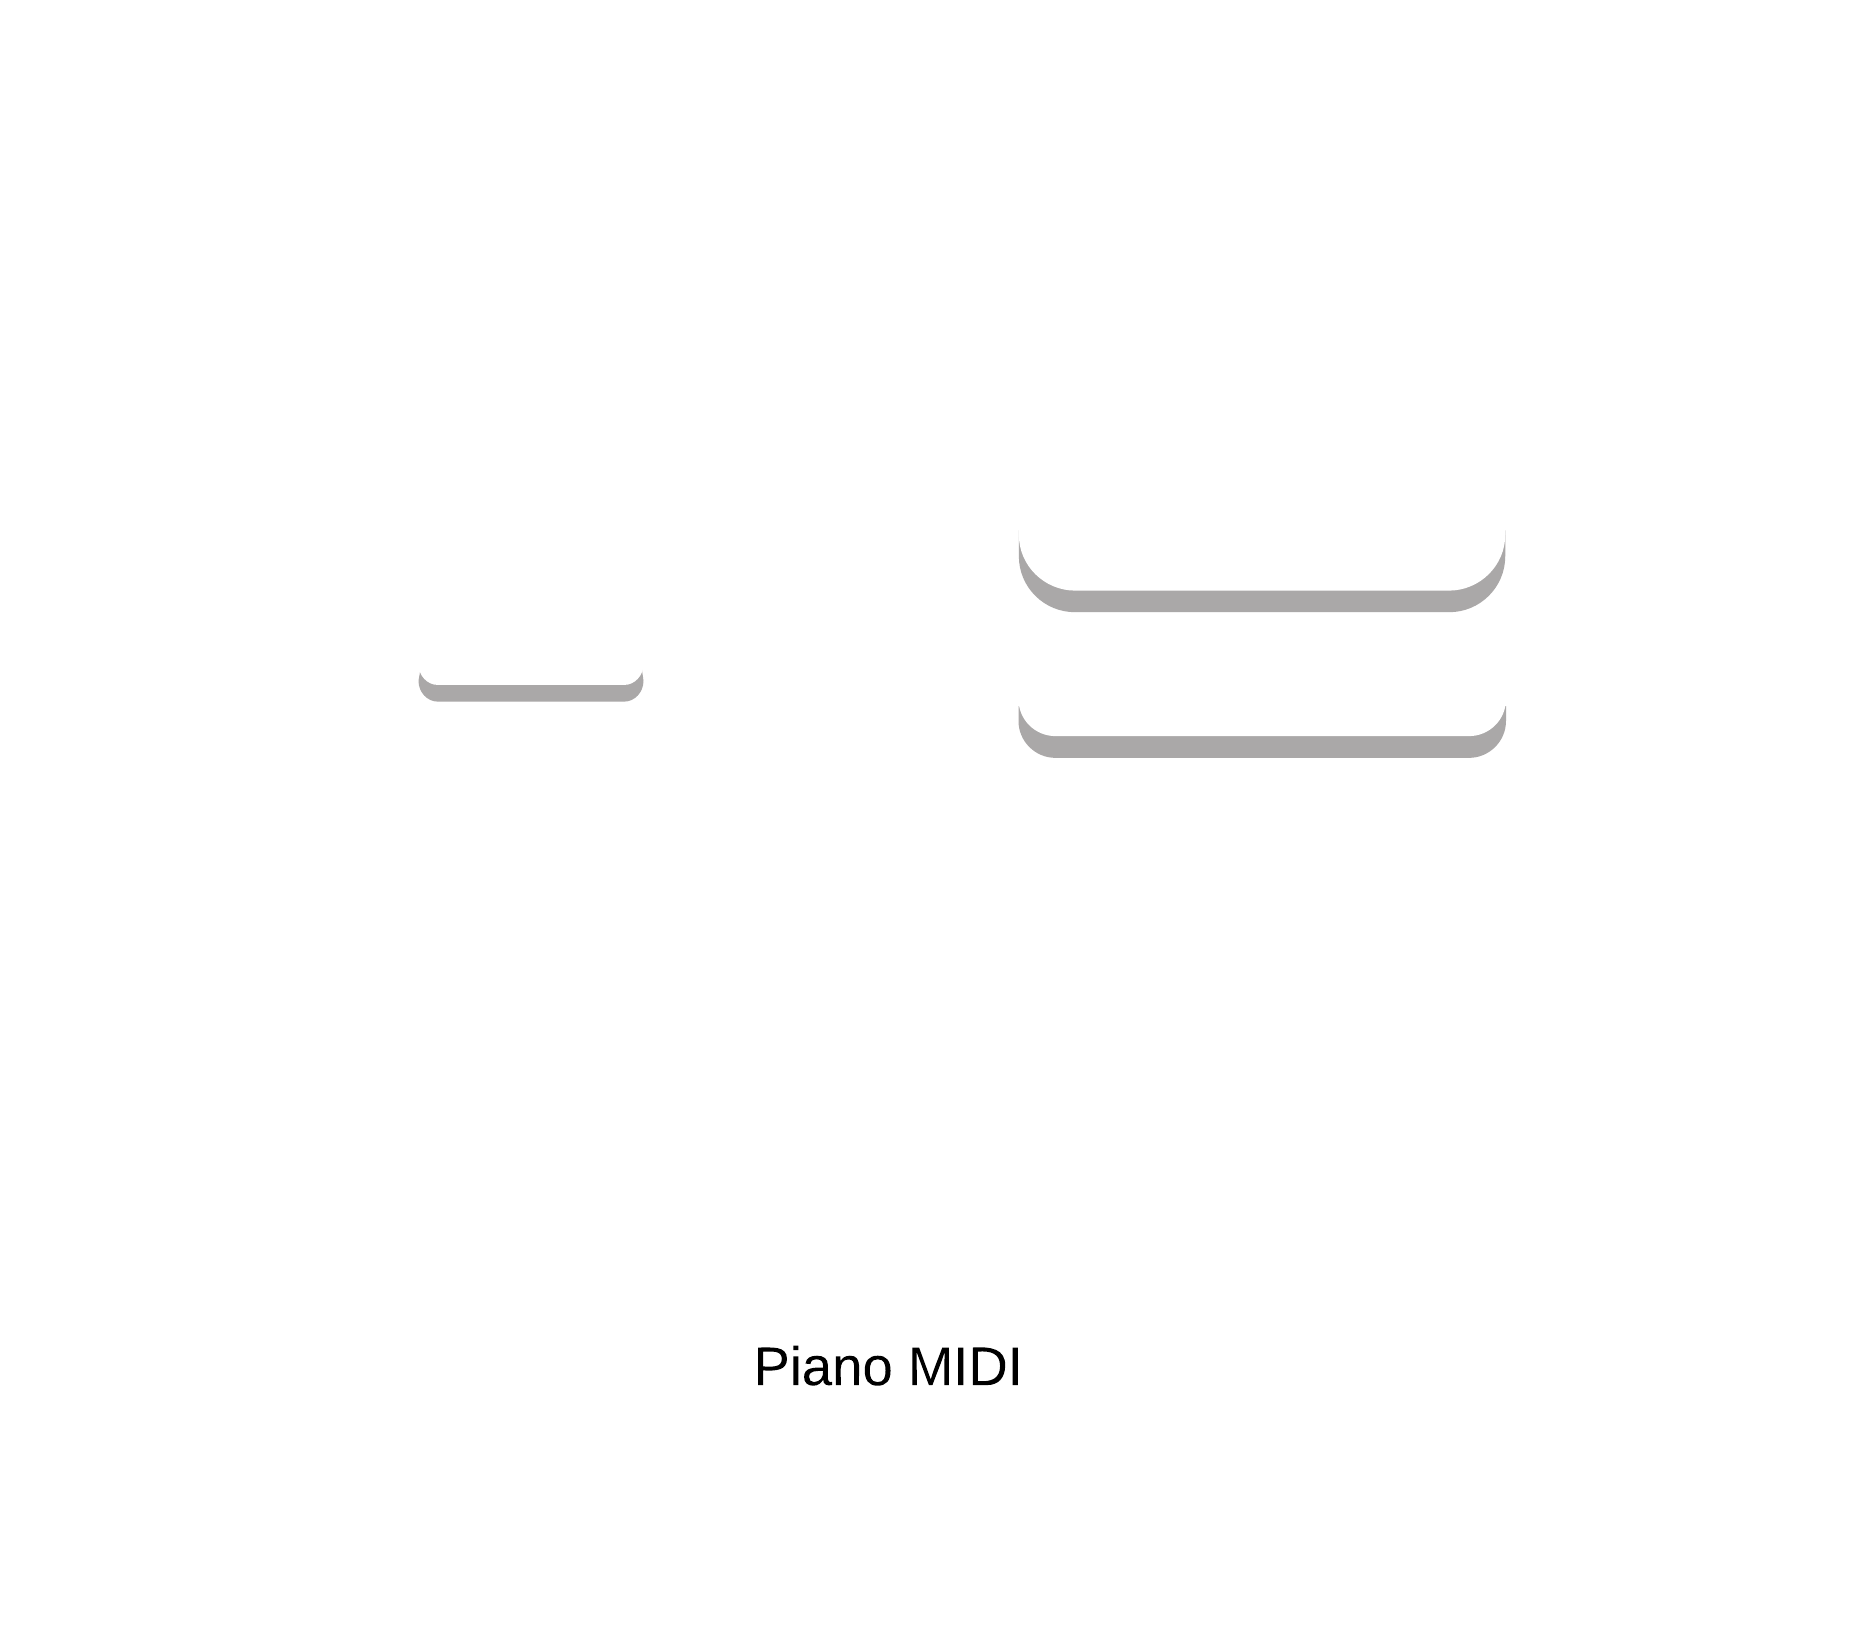
\includegraphics[width=\textwidth]{../assets/structure-front.png}

Pour fonctionner, ChromaCase récupère les notes que vous jouez sur votre Piano et les évalue en temps réel. 

\subsection{Installation \& Acces}

Avant de vous rendre sur ChromaCase, branchez votre piano à votre appareil.

Si vous utilisez un navigateur, vous devriz surement autoriser ChromaCase à accéder aux connections MIDI.

Pour accéder à Chromacase, rendez-vous sur \url{https://chroma.octohub.app/}. Vous arriverez sur la page d'accueil, depuis laquelle vous devrez vous authentifier (ou créer un compte) pour continuer (cf section Guide d'utilisation)
